\section{提案手法}
\label{sec:Proposed}
本研究はDPDKのRun-to-Completionモデルを用いたL2分散計算環境を提案する.本章では,その概要としてDPDKによるL2通信を用いることとRun-to-Completionモデルで処理を実行することについて述べる.

\subsection{DPDKによるL2通信を用いる}
第\ref{sec:Problem}章で述べたとおり,TCP/IPによる通信ではルーティング,誤り制御,順序制御といった制御が行われる.しかし,第\ref{sec:Background}章で述べた本研究が提案する分散計算環境の前提を踏まえると,これらの制御は本研究においてはオーバーヘッドである.また,カーネルによるパケットI/Oには,一定時間に受信するパケットの量が増えると,コンテキストスイッチが増加して,割り込み以外の処理が実行できなくなってしまう問題がある.また,ユーザ空間のアプリケーションがパケットにアクセスするには,受信したパケットをカーネル空間からユーザ空間にコピーしなければならない問題もある.これらの問題により,カーネルのパケットI/OはDPDKのパケットI/Oに比べて低速である.

そこで,本研究では分散計算環境の計算機間の通信にDPDKによるL2通信を用いる.これによって,TCP/IPによる通信のオーバーヘッドをなくすことができる.また,カーネルによるパケットI/Oに比べて高速なパケットI/Oを用いることもできる.

\subsection{Run-to-Completionモデルで処理を実行する}
第\ref{sec:DPDK}章で述べたとおり,DPDKのPipelineモデルは受信処理,パケット処理,送信処理をそれぞれ別の論理コアで行うため,コアの使用効率が悪い問題とCPUのL1キャッシュを有効活用できない問題がある.また,DPDKは特定のCPUコアを専有することによって,NICを常時ポーリングで監視するため,通信スループットが低いときでもCPUリソースを無駄に使ってしまう問題もある.

そこで,本研究では計算機をメッシュネットワークで接続し,Run-to-Completionモデルで処理を実行する(図\ref{fig:Proposed}).受信処理,パケット処理,送信処理を一つの論理コアで行うRun-to-Completionモデルを用いることで,Pipelineモデルを用いる場合に比べて多くの計算機と接続することができ,コアを有効活用できる.また,本研究が提案する分散計算環境の計算機間でやり取りされるデータのサイズはL2フレームの1.5KBより小さいため,CPUのL1キャッシュを有効活用できる.さらに,メッシュネットワークで接続された計算機が協調して処理を実行することによって,通信スループットが低い状態にならず,CPUリソースを有効活用できる.

\begin{figure}[htb]
  \centering
  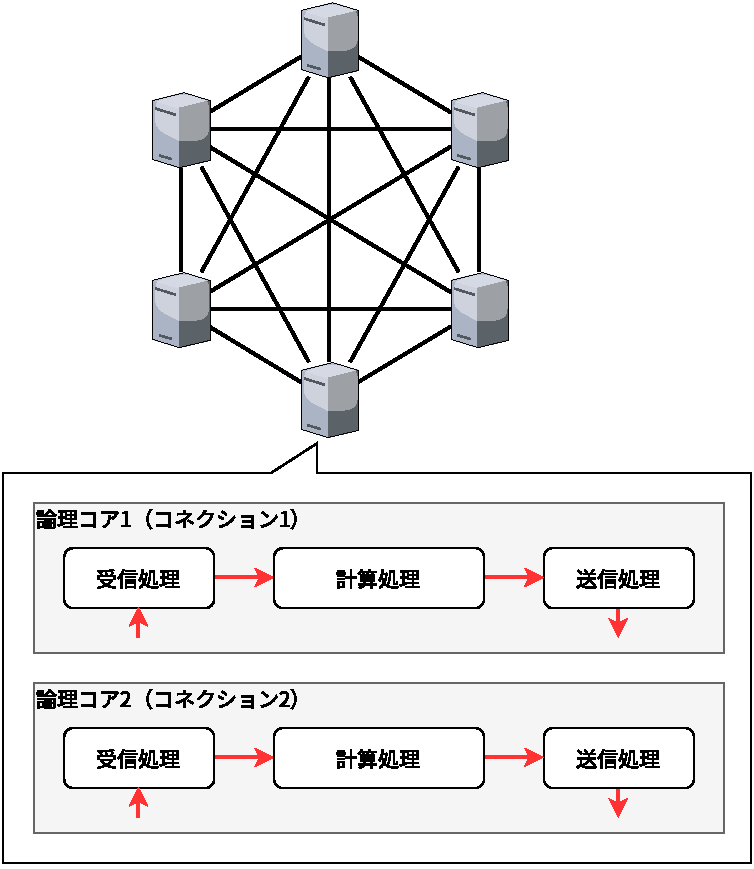
\includegraphics[width=\columnwidth]{pictures/Proposed.pdf}
  \caption{提案手法}
  \label{fig:Proposed}
\end{figure}
